% Template for Cogsci submission with R Markdown

% Stuff changed from original Markdown PLOS Template
\documentclass[10pt, letterpaper]{article}

\usepackage{cogsci}
\usepackage{pslatex}
\usepackage{float}
\usepackage{caption}

% amsmath package, useful for mathematical formulas
\usepackage{amsmath}

% amssymb package, useful for mathematical symbols
\usepackage{amssymb}

% hyperref package, useful for hyperlinks
\usepackage{hyperref}

% graphicx package, useful for including eps and pdf graphics
% include graphics with the command \includegraphics
\usepackage{graphicx}

% Sweave(-like)
\usepackage{fancyvrb}
\DefineVerbatimEnvironment{Sinput}{Verbatim}{fontshape=sl}
\DefineVerbatimEnvironment{Soutput}{Verbatim}{}
\DefineVerbatimEnvironment{Scode}{Verbatim}{fontshape=sl}
\newenvironment{Schunk}{}{}
\DefineVerbatimEnvironment{Code}{Verbatim}{}
\DefineVerbatimEnvironment{CodeInput}{Verbatim}{fontshape=sl}
\DefineVerbatimEnvironment{CodeOutput}{Verbatim}{}
\newenvironment{CodeChunk}{}{}

% cite package, to clean up citations in the main text. Do not remove.
\usepackage{cite}

\usepackage{color}

% Use doublespacing - comment out for single spacing
%\usepackage{setspace}
%\doublespacing


% % Text layout
% \topmargin 0.0cm
% \oddsidemargin 0.5cm
% \evensidemargin 0.5cm
% \textwidth 16cm
% \textheight 21cm

\title{Drawings as a window into developmental changes in object
representations}


\author{{\large \bf Bria Long} \\ \texttt{bria@stanford.edu} \\ Department of Psychology \\ Stanford University \And {\large \bf Judith E. Fan} \\ \texttt{jefan@stanford.edu} \\ Department of Psychology \\ Stanford University \And {\large \bf Michael C. Frank } \\ \texttt{mcfrank@stanford.edu} \\ Department of Psychology \\ Stanford University}

\begin{document}

\maketitle

\begin{abstract}
How do object category representations change throughout childhood? To
approach this question, we turned to drawings as a way to investigate
children's internal representations of object categories. We asked
children (ages 3-10 years) to draw a wide range of objects (e.g. `can
you draw a chair?') in under 30 seconds. Then, we analyzed how the
content of these drawings changes across development. We analyzed the
degree to which children were able to depict recognizable exemplars of
these categories, and found that children become increasingly skilled at
producing recognizable drawings, even when controlling for low-level
covariates (the amount of ink used, the time spent drawing, and the
number of strokes). Second, we analyzed the degree to which children's
drawings share perceptual features with those produced by adults,
analyzing their featural similarity at each layer of deep convolutional
neural network. Overall, we find that childrens' drawings were most
similar to adults' in higher-level layers of the network. These results
suggest that the ability to produce abstract graphical represnetations
of objects is highly developed by middle childhood, and that even the
most primitive drawings made by children contain featural similarities
to the objects they are trying to depict. Broadly, these results point
towards drawing as a promising avenue for investigating object
representations in childhood.

\textbf{Keywords:}
object representations; drawings; child development
\end{abstract}

\section{Introduction}\label{introduction}

Consider what one has to do in order to draw ``a phone'' -- one needs to
access the mental representation of ``a phone'', distill this into a
pictoral format, and plan a sequence of hand movements to effectively
convey this visual concept. Yet this is a trivial task for adults. How
do children's drawings change over development? And might they offer a
window into how young children represent object categories?

While drawing has been extensively studied in early childhood, a primary
focus has been on when children come to treat drawings as symbols for
object categories (Gardner, 1994). And a wealth of evidence now suggests
that in fact young children attribute rich meanings to their drawings.
For example, children will attribute different symbolic content (e.g.,
``a balloon'', ``a lollipop'') to very similar drawings based on what
they intended to draw (Bloom \& Markson, 1998). Further, children will
monitor whether their drawings are adequate symbols for the things they
are trying to draw, and will improve their drawings when given feedback
that their drawings are not effective at communicating the identity of
object (Callaghan, 1999).

Far less research, however, has examined if children's drawings reflect
how children represent objects in the world around them. Indeed,
drawings are a powerful way to tap internal representations of object
categories, even in non-expert adults. For example, adults tend to draw
objects relative to their size in the real-world: objects that are big
in the real-world (e.g., cars) tend to take up more ``space'' on a
canvas than objects that are small in the real-world (e.g., cups)
(Konkle \& Oliva (2011)). Moreover, to be recognizable, drawings have to
depict the necessary features to express a given visual concept. This
intuition is supported by recent computational work: deep neural network
models of the ventral stream trained purely on photographs can also
recognize drawings by non-expert adults, as drawings and photographs
generate similar representations in higher-level layers of these models.
In other words, drawings capture high-level similarity relationships
between object categories (Fan, Yamins, \& Turk-Browne, 2015).

Some evidence suggests that children's ability to recognize objects
continues to develop into early adolescence, including the ability to
recognize objects across dramatic changes in viewpoint (Bova et al.,
2007; Dekker, Mareschal, Sereno, \& Johnson, 2011). Children's ability
to process the relationship between objects' parts also has a protracted
developmental trajectory (for reviews, see Nishimura, Scherf, \&
Behrmann (2009); Jüttner, Wakui, Petters, \& Davidoff (2016)). For
example, while young children have a bias to categorize novel objects on
the basis of part-specific information, older children rely more on the
relationship between the object parts (Mash, 2006); and even older
children have difficulty detecting changes in the propotions of an
object's parts in familiar categories (i.e., animals; (Davidoff \&
Roberson, 2002; Jüttner, Petters, Wakui, \& Davidoff, 2014; Jüttner,
Wakui, Petters, Kaur, \& Davidoff, 2013)). Thus, this work raises the
possibility that children's representations of common object categories
(e.g., cups, cars) are also undergoing developmental changes. In
general, however, there is a lack of behavioral research systematically
examining object category representations in childhood and comparing
them to those of adults.

Here, we use children's drawings as window into object representations
in childhood. First, we ask if children produce more recognizable
drawings as they get older after factoring out low-level covariates.
Second, we examine how similar children and adult's drawings are in
terms of their perceptual features by comparing their representations in
a deep convolutional neural network (VGG-19). We conclude b

\section{Part 1: Why do children get better at
drawing?}\label{part-1-why-do-children-get-better-at-drawing}

First, children (ages 3-10 years) produced drawings of 16 common object
categories in a simple drawing game. Then, naïve adults attempted to
recognize these drawings in a forced-choice recognition task.

\begin{CodeChunk}
\begin{figure*}[h]

{\centering 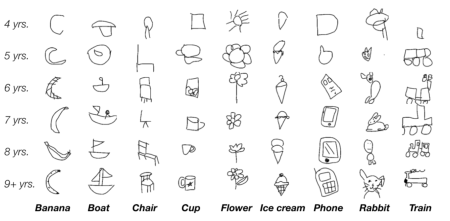
\includegraphics[width=1\linewidth]{figs/exampleDrawings-1} 

}

\caption[Example drawings made by children ages 4-10 of several object  categories]{Example drawings made by children ages 4-10 of several object  categories.}\label{fig:exampleDrawings}
\end{figure*}
\end{CodeChunk}

\subsection{Methods}\label{methods}

\subsubsection{Participants}\label{participants}

For the drawing task, children (N = 41, M = 6.9 years, range 4-10 years)
were recruited at the San Jose Children's Discovery Museum and
participated in this experiment. For the recognizability experiment, 14
adults with US IP addresses were recruited and rated all of the 268
drawings.

\subsubsection{Materials}\label{materials}

We implemented a simple drawing game in HTML/Javascript using the
paper.js library; this web-based experiment was run on an iPad on the
floor of the museum. All code is available at
www.github.com/brialorelle/kiddraw/museumdraw.

\subsubsection{Drawing Game Procedure}\label{drawing-game-procedure}

On each trial, a text cue would appear (i.e., ``Can you draw a
{[}flower{]}?'') that the experimenter would read out, (``What about a
{[}flower{]}? Can you draw a {[}flower{]}?). Then, a drawing canvas
appeared (600 x 600 pixels) and children were had 30 seconds to make a
drawing before the game moved on to the next trial. After each trial,
the experimenter asked the child whether they wanted to keep drawing or
whether they were all done. On the first two trials of the experiment,
every child was prompted to draw the same two common shapes----a circle
and a triangle. These trials served to familiarize children with the
drawing task and to practice using their fingers to draw.

\subsubsection{Stimuli}\label{stimuli}

Stimuli were words referring to 16 common object categories (banana,
boat, car, carrot, cat, chair, couch, cup, flower, foot, frog, ice
cream, phone, rabbit, shoe, train). These categories were chosen such
that they were (1) likely to be familiar to children, (2) present in the
Google QuickDraw database, (3) spanned the animate/inanimate distinction
and (4) intuitively spanned a wide range of difficulty (for example,
flowers seem easier to draw than couches).

\subsubsection{Recognizability Task}\label{recognizability-task}

14 naïve adults assessed the recognizability of all of the 286 drawings
produced by these children. On each trial, participants saw a drawing,
and were asked ``What does this look like?'', and responded by typing
into a text box; participants could then choose between 21 possible
answers. 16 of these possible answers were the original object
categories; however, we also included five additional foil items (bean,
arm, person, rock, and ``cannot tell at all''). All drawings were
presented in a random order, and participants were not informed that
these drawings were produced by children or the context in which they
were produced. An answer was scored as ``correct'' if adults were able
to correctly guess the object category that children were cued with.

\subsubsection{Low-level covariates.}\label{low-level-covariates.}

The use of a digital interface for drawing allowed us to quickly and
easily assess the contribution of several low-level factors that may
co-vary with drawing ability. For each drawing, we thus quantified the
amount of time spend drawing, the number of strokes used, and the
overall intensity of the drawing(e.g., amount of ink). Descriptives
plots describing the output of these variables can be seen in (see
Figure \ref{fig:covDescriptives}, left).

\subsubsection{GLMM procedure.}\label{glmm-procedure.}

We aimed to assess whether children's ability to produce recognizable
drawings increased with age, independent of low-level covariates. To do
so, we used a generalized logistic mixed effect model, with age, drawing
duration, amount of ink used, and number of strokes as fixed effects,
and with random effects for each individual child drawer and object
category. The dependent variable was whether the proportion of adults
that recognized a given drawing. This was specified in the lme4 r
package as: glmer(correct \textasciitilde{} scale(age) +
scale(draw\_duration) + scale(mean\_intensity) + scale(num\_strokes)
+(1\textbar{}session\_id) + (1\textbar{}category), family =
``binomial'')

\subsection{Results}\label{results}

\begin{CodeChunk}
\begin{figure}[H]

{\centering 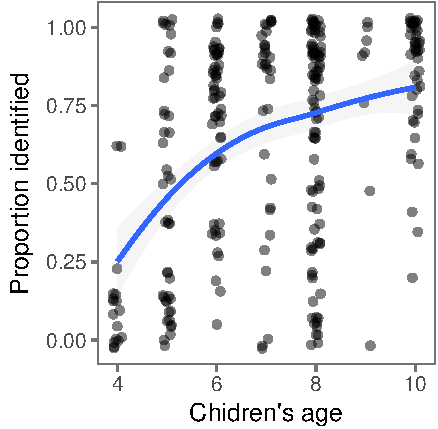
\includegraphics{figs/recByAge-1} 

}

\caption[Drawings are plotted according to the age of the drawer (x-axis) and the proportion of adults that correctly identified the target object category in recognition task (y-axis)]{Drawings are plotted according to the age of the drawer (x-axis) and the proportion of adults that correctly identified the target object category in recognition task (y-axis); each dot represents one drawing.}\label{fig:recByAge}
\end{figure}
\end{CodeChunk}

\begin{CodeChunk}
\begin{figure}[H]

{\centering 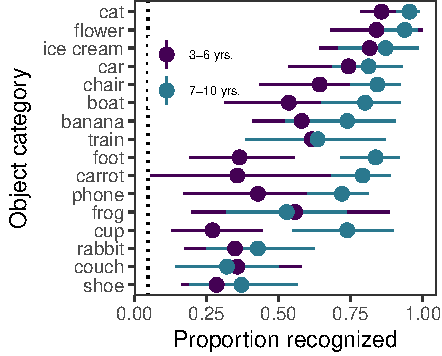
\includegraphics{figs/recognizabilityByItem-1} 

}

\caption[Proportion of drawings recognized for object category, sorted from hardest to easiest items]{Proportion of drawings recognized for object category, sorted from hardest to easiest items. Error bars represent non-parametric 95 percent confidence intervals, estimated using the langcog r package.}\label{fig:recognizabilityByItem}
\end{figure}
\end{CodeChunk}

First, we observed that some items were much easier to draw than others.
For example, children of all ages produced drawings of cats that were
readily recognizable as ``cats'', but few children of any age produced
drawings that were recognizable as ``shoes'' (see Figure
\ref{fig:recognizabilityByItem}). Howver, almost all items also saw an
increase in recognizability with the age of the drawer. Across all
items, the proportion of drawings recognized increased steadily with age
(see Figure \ref{fig:recByAge}).

Next, we asked whether this relationsip persists when we control for
low-level covariates: the number of strokes, amount of ink used, and the
time spent drawing. In other words, is this increase in recognizability
due to an increase in expressive power, or simply due to the fact that
older children may have put more effort into their drawings? Our
generalized logistic mixed-effect model revealed that the
recognizability of drawings increased reliably with when controlling for
these low-level covariates --- the amount of time spent drawing, the
number of strokes, and total ink used (b = 0.96, SE = 0.17, Z = 5.5),
and accounting for variation across object categories and individual
children. All model coefficients can be seen in Table 1.. Adding
interaction terms between age and these low-level covariates did little
to decrease the effect of age on recognizability (b = 0.94, SE = 0.18, Z
= 5.4). Thus, these results suggest that the ability to quickly produce
graphical representations of object categories increases with age,
controlling for low-level covariates. Further, these results sugest that
this ability is highly developed by middle childhood.

\begin{CodeChunk}
\begin{figure*}[h]

{\centering 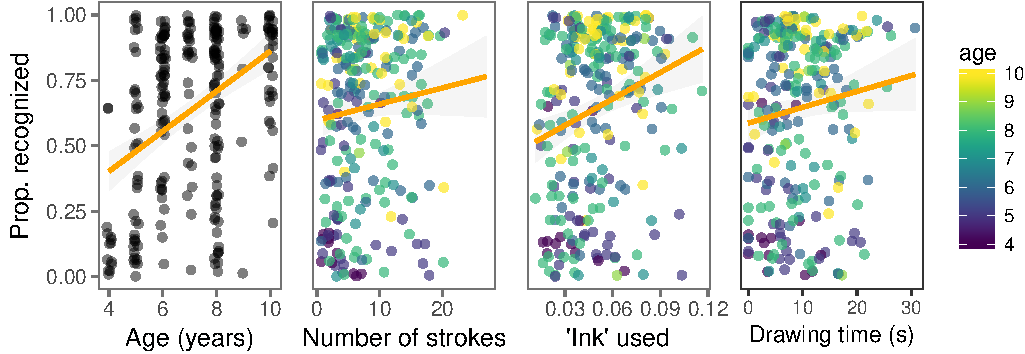
\includegraphics{figs/covDescriptives-1} 

}

\caption[The proportion of adults who recognized each drawing is plotted as a function of the number of strokes, amount of ink used, and the time spent creating each drawing]{The proportion of adults who recognized each drawing is plotted as a function of the number of strokes, amount of ink used, and the time spent creating each drawing. Each dot represents an individual drawing; dots are colored by the age of the drawer.}\label{fig:covDescriptives}
\end{figure*}
\end{CodeChunk}

\begin{table}[H]
\centering
\begin{tabular}{rrrrr}
  \hline
 & Estimate & Std. Error & z value & Pr($>$$|$z$|$) \\ 
  \hline
(Intercept) & 0.861 & 0.321 & 2.680 & 0.007 \\ 
  Age & 0.956 & 0.174 & 5.497 & 0.000 \\ 
  Drawing time & 0.338 & 0.109 & 3.105 & 0.002 \\ 
  Amount of ink & 0.014 & 0.080 & 0.179 & 0.858 \\ 
  Num. strokes & -0.289 & 0.098 & -2.959 & 0.003 \\ 
   \hline
\end{tabular}
\caption{Model coefficients of a GLMM predicting the recognziability of each  drawing.} 
\end{table}

\section{Part 2: How similar are children's and adult's
drawings?}\label{part-2-how-similar-are-childrens-and-adults-drawings}

To what degree are children's drawings similar to those of adults? While
younger children often produced drawings that were unrecognizable at the
basic-level, these recognizability ratings may underestimate the
perceptual content depicted in children's drawings. For example,
children may not be able to depict the visual differences between a
bunny and a frog, but they still may capture many of the essential
perceptual features needed to depict an animal. Here, we turn to deep
neural network models of object recognition to quantify the similarities
between children's and adults drawings, asking how similar they are in
terms of feature similarity at each progressively complex layer of a
deep convolutional neural network (Simonyan \& Zisserman, 2014). In
other words, how similar are children and adult's drawings (and why)?

For this analyses, we collected a larger sample of drawings using the
same methodology, this time sampling from both the previously used
categories as well as a new selection of 22 categories (see Stimuli)
allowing us to span superordinate category distinctions. With this
larger sample of drawings, we thus examine the degree to which children
and adults drawings resemble each other in a deep convolutional neural
network, specifically VGG-19.

\subsection{Methods}\label{methods-1}

\subsubsection{Stimuli}\label{stimuli-1}

For this second round of data collection, we expanded our set of
categories to include equal numbers of vehicles, furniture, small
objects, food items, mammals, and non-mammals (new items: airplane, bus,
bike, piano, table, door, bed, fork, keys, hat, apple, cookie, mushroom,
horse, dog, sheep, bear, fish, bird, spider, shark, duck).

\subsubsection{Participants}\label{participants-1}

Participants included those who participated in the first round of data
collection, used in Experiment 1, as well as an additional 37 children,
again recruited from the floor of the San Jose Children's Discovery
Museum. Overall, this yielded an additional 98 drawings (excluding
practice trials) for a total of 387 drawings. For the subsequent
analyses, we binned children's age coarsely into ``younger children''
(aged 3-6 years) and ``older'' children (aged 7-10 years) and restricted
analyses to categories where we had at least 3 drawings per age group
(16 categories); this allowed us to analyze approximately the same
number of drawings in each age group (younger children, N=118 drawings;
older children, N=161 drawings). This ensured the robust estimates of
feature distance in the folowing analyses.

\subsubsection{Adult drawings}\label{adult-drawings}

We obtained a sample of adult drawings from the Google QuickDraw
database. Specifically, we randomly sampled 1000 images for each object
category, irrespective of any information about the adult drawer or the
quality of the drawing. See \url{https://quickdraw.withgoogle.com/data}
for visualizations of this dataset.

\subsubsection{Convolutional Neural Network (CNN)
Features}\label{convolutional-neural-network-cnn-features}

We used a standard, pre-trained implementation of VGG-19 (Simonyan \&
Zisserman, 2014) to extract features in response to all sketches at each
layer of the network, including the first five convolutional layers
(C1-C5) as well as the two fully-connected layers (FC6 and FC7).
Features were normalized within each layer across all sketches and then
averaged within each category (e.g., ``cat'', ``rabbit''). This yielded
a vector corresponding to the number of features in each layer for all
38 of the drawn categories in younger children, older children, and
adults.

\subsubsection{Representational Similarity
Analyses}\label{representational-similarity-analyses}

Separately for drawings from younger children, older children, and
adults, we averaged the feature vectors within each object class for a
given layer of VGG and then computed a layer-specific matrix of the
Pearson correlation distances between these average vectors across
classes (Kriegeskorte et al., 2008). Formally, this entailed computing:
\[RDM(R)_{ij} = 1- \frac{cov(\vec{r}_{i}, \vec{r}_{j})}{\sqrt{var(\vec{r}_{i}) \cdot var(\vec{r}_{j})}}\],
where \(\vec{r}_{i}\) and \(\vec{r}_{j}\) are the mean feature vectors
for the \(i\)th and \(j\)th object classes, respectively. Each of these
16x16 representational dissimilarity matrices (RDMs, shown in Figure
\ref{fig:RSAAllCat}) provides a compact description of the layout of
objects in the high-dimensional feature space inherent to each layer of
the model. Following Kriegeskorte et al. (2008), we measured the
similarity between object representations in different layers by
computing the Spearman rank correlations between the RDMs for those
corresponding layers.

Estimates of standard error for the Spearman correlation between RDMs
(i.e., between domains or between layers) were generated by jackknife
resampling of the 16 object classes. This entails iterating through each
of the 16 subsamples that exclude a single class, computing the
correlation on each iteration, then aggregating these values.
Specifically, the jackknife estimate of the standard error can be
computed as:
\(s.e._{(jackknife)} = \sqrt{\frac{n-1}{n} \sum_{i=1}^{n} (\bar{x}_{i} - \bar{x}_{(.)})^{2}}\),
where \(\bar{x}_{i}\) is the correlation based on leaving out the
\(i\)th object class and
\(\bar{x}_{(.)} = \frac{1}{n} \sum_{i}^{n} \bar{x}_{i}\), the mean
correlation across all subsamples (of size 15). This estimate of
standard error allows us to construct 95\% confidence intervals and
compute two-sided p-values for specific comparisons (Efron, 1979; Tukey,
1958).

\subsubsection{Category similarity
analyses}\label{category-similarity-analyses}

We also directly analyzed the similarity of the feature representations
generated by sketches from younger children vs.~adults and between older
children vs.~adults. To do so, we computed the Pearson correlation
between the average category vectors for adults and the average category
vectors for younger/older children (separetly). This yielded a
correlation score for each object category for each age comparison.

\subsubsection{Category classification
analyses}\label{category-classification-analyses}

Model features were also used to train softmax classifiers
(\url{http://scikit-learn.org/}) with L2 regularization to evaluate the
degree to which category information was linearly accessible from
sketches made by each group of participants. Predictions are then made
for images held out from the training set, and accuracy is assessed on
these held-out images. The robustness of classifier accuracy scores was
determined using stratified 5-fold cross validation on 80\% train/20\%
test class-balanced splits.

\begin{CodeChunk}
\begin{figure*}[h]

{\centering 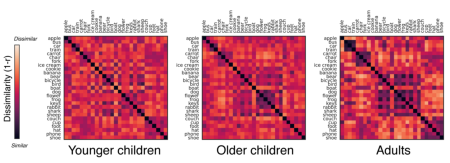
\includegraphics{figs/RSAAllCat-1} 

}

\caption[Representational dissimilarity matrixes (RDMs) in the highest layer of VGG-19 (FC7) for drawings made by younger children ( 3-6 years of age), older children (7-10 years of age), and adults (Google QuickDraw database)]{Representational dissimilarity matrixes (RDMs) in the highest layer of VGG-19 (FC7) for drawings made by younger children ( 3-6 years of age), older children (7-10 years of age), and adults (Google QuickDraw database). Each square in one of these matrixes represnets the correlation distance between two categories (e.g., chair and couch) in this layer of the network; lighter colors indicate pairs of categories that generated dissimilar feature representations; darker colors indicate pairs of cateogries that generated more similar feature representations. Categories are grouped to reveal the inherent simiarity structure.}\label{fig:RSAAllCat}
\end{figure*}
\end{CodeChunk}

\subsection{Results}\label{results-1}

\subsubsection{Layer-wise feature
similarity}\label{layer-wise-feature-similarity}

We first examined the featural similarities between sketches produced by
adults and children at each layer of VGG-19. Overall, we found that the
similarity between older children and adults' drawings increased in each
subsequent layer of the network, reaching a peak in the final layers of
the network (see Figure \ref{fig:layerWise}; Spearman's r values, Layer
1=0.215, Layer 2=0.206, Layer 3=0.249, Layer 4=0.435, Layer 5=0.637,
Layer 6=0.696, Layer 7=0.72). For younger children, we found a similar
pattern of results, though similarity to adult drawings was overall
lower (Spearman's r values, Layer 1=0.074, Layer 2=0.001, Layer 3=0.04 ,
Layer 4=0.119, Layer 5=0.368, Layer 6=0.464, Layer 7=0.49). The RDMs for
the final layer of the network (where similarity was the highest; FC7)
are shown in Figure \ref{fig:RSAAllCat} for younger children, older
children, and adults.

\begin{CodeChunk}
\begin{figure}[H]

{\centering 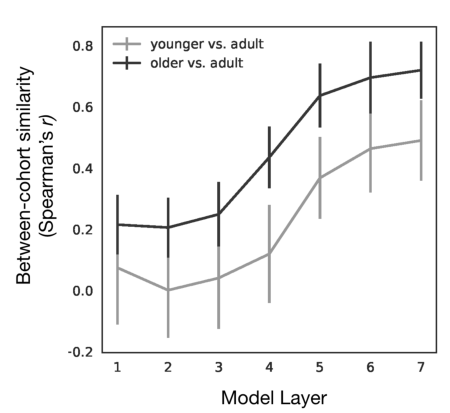
\includegraphics{figs/layerWise-1} 

}

\caption[Spearman's correlation between representational dissimilarity matrixes (RDMs) between drawings produced by adults and younger children (grey line) and between adults and older children (black line) at each layer of VGG-19--the first five convolutional layers and the last two fully connected layers]{Spearman's correlation between representational dissimilarity matrixes (RDMs) between drawings produced by adults and younger children (grey line) and between adults and older children (black line) at each layer of VGG-19--the first five convolutional layers and the last two fully connected layers. Error bars represent standard error of the mean obtained by a jacknife re-sampling procedure (see Methods).}\label{fig:layerWise}
\end{figure}
\end{CodeChunk}

\subsubsection{Category similarity
analyses}\label{category-similarity-analyses-1}

Next, we explored which categories generated representations in FC7 that
were more or less similar between younger children vs.~adults and
between older children vs.~adults (see Figure \ref{fig:simpleCorr}).
Overall, we found a good deal of variability; for some categories,
children's and adults drawings had feature representatinos that were
relatively dissimilar (e.g., couches, shoes) while others generated very
similar feature representations (e.g., flowers, chairs) in this final
layer of the network.

\begin{CodeChunk}
\begin{figure}[H]

{\centering 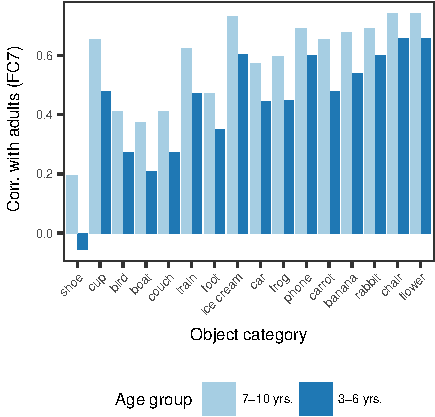
\includegraphics{figs/simpleCorr-1} 

}

\caption[Spearman's correlation between children's and adults sketches in layer FC7 for each object category]{Spearman's correlation between children's and adults sketches in layer FC7 for each object category.}\label{fig:simpleCorr}
\end{figure}
\end{CodeChunk}

\subsubsection{Classification results}\label{classification-results}

Finaly, we examined the degree to which these featural representations
could be used to classify these skeches at the basic-level. We found
that sketches made by younger children were classifiable 35\% of the
time (SD=5\%), while those made by older children (7-10 years) were
classifiable 51\% of the time (SD=6\%). While the overall performance of
the classified is relatively low compared to the human performance seen
in Part 1, we still observed a relative increase in recognizability
between younger and older children. Thus, these results suggest that the
difference in recognizability of the sketches stems directly from a
differences in perceptual features that can be detected by a deep
convolutional neural network trained to recognize objects.

Taken together, these results suggest that children and adults are
accessing similar category representations to perform these drawing task
that manifest in perceptual similarities between adults and children,
even in the most primitive drawings.

\section{General Discussion}\label{general-discussion}

We explored how children get better at drawing and how similar their
drawings are to adults'. Overall, we found that the capacity to quickly
produce graphical representations that communicate object category
information is highly developed by middle childhood. Children produced
drawings in under 30 seconds that were recognizable by adults with only
the few ``strokes'' of a pen; older children were better able to produce
these graphical abstractions than younger children, irrespective of the
amount of time they spent drawing or the amount of ``ink'' they used.
Further, children's drawings were most similar to adult drawings in the
higher-level layers of a deep convolutional neural network trained to
recognize objects, suggesting that children and adults drawings share
high-level perceptual features useful for basic-level object
recognition.

An obvious future direction concerns the contribution of children's
motor control to their drawing abilities. In other words, to what degree
are drawings made by older children more recognizable simply because
older children have better fine motor control? Children certainly
practice drawing----both on their own and in structured settings (e.g.,
art classes)--and this practice invariably plays a role in the fidelity
of drawings that children can produce. We plan to measure children's
fine motor control on an orthogonal task (e.g., tracing a complex shape)
to begin to understand how this factor influences the recognizability of
children's drawings.

Ultimately, we hope to understand the degree to which changes in
children's drawings of object categories reflect changes in children's
representations of object categories. Throughout childhood, children
certainly acquire a wealth of experience with the objects in the world
around them, and this experience likely helps build more detailed
internal representations of the categories. Thus, one possibility is
that children's internal representations that they map to the words
``rabbit'', ``chair'', and ``couch'' are becoming more detailed as they
grow older, and that it is these more detailed representations that, in
turn, feed into their rapid drawings of these object categories. If this
is the case, then children's abilities to depict certain object
categories may patterns with their object categorization errors. For
example, older (vs.~younger) children may be better able to draw cats
vs.~rabbits and better able to distinguish between cats vs.~rabbits.
Future work that links children's categorization abilities with their
visual production behaviors may begin to answer this question.

In sum, this work begins a developmental project examining children's
object representations using a common production task--drawing. An
understanding of how we produce efficient graphical abstractions of the
objects in our everyday world may help uncover the building blocks of
our object category representations.

\section{Acknowledgements}\label{acknowledgements}

We gratefully acknowledge those who made the Google QuickDraw database
avaliable. This work was funded by a \#\# to Judy Fan, and a \#\#\# to
Michael C. Frank, and a \#\#\# to Bria Long.

\section{References}\label{references}

\setlength{\parindent}{-0.1in} \setlength{\leftskip}{0.125in} \noindent

\hypertarget{refs}{}
\hypertarget{ref-bloom1998intention}{}
Bloom, P., \& Markson, L. (1998). Intention and analogy in children's
naming of pictorial representations. \emph{Psychological Science},
\emph{9}(3), 200--204.

\hypertarget{ref-bova2007}{}
Bova, S. M., Fazzi, E., Giovenzana, A., Montomoli, C., Signorini, S. G.,
Zoppello, M., \& Lanzi, G. (2007). The development of visual object
recognition in school-age children. \emph{Developmental
Neuropsychology}, \emph{31}(1), 79--102.

\hypertarget{ref-callaghan1999early}{}
Callaghan, T. C. (1999). Early understanding and production of graphic
symbols. \emph{Child Development}, \emph{70}(6), 1314--1324.

\hypertarget{ref-davidoff2002}{}
Davidoff, J., \& Roberson, D. (2002). Development of animal recognition:
A difference between parts and wholes. \emph{Journal of Experimental
Child Psychology}, \emph{81}(3), 217--234.

\hypertarget{ref-dekker2011dorsal}{}
Dekker, T., Mareschal, D., Sereno, M. I., \& Johnson, M. H. (2011).
Dorsal and ventral stream activation and object recognition performance
in school-age children. \emph{NeuroImage}, \emph{57}(3), 659--670.

\hypertarget{ref-Efron:1979ts}{}
Efron, B. (1979). 1977 Rietz Lecture - Bootstrap Methods - Another Look
at the Jackknife. \emph{Annals of Statistics}, \emph{7}(1), 1--26.

\hypertarget{ref-fan2015common}{}
Fan, J. E., Yamins, D., \& Turk-Browne, N. B. (2015). Common object
representations for visual recognition and production. In \emph{CogSci}.

\hypertarget{ref-gardner1994arts}{}
Gardner, H. (1994). \emph{The arts and human development: With a new
introduction by the author}. Basic Books.

\hypertarget{ref-juttner2014late}{}
Jüttner, M., Petters, D., Wakui, E., \& Davidoff, J. (2014). Late
development of metric part-relational processing in object recognition.
\emph{Journal of Experimental Psychology: Human Perception and
Performance}, \emph{40}(4), 1718.

\hypertarget{ref-juttner2016developmental}{}
Jüttner, M., Wakui, E., Petters, D., \& Davidoff, J. (2016).
Developmental commonalities between object and face recognition in
adolescence. \emph{Frontiers in Psychology}, \emph{7}.

\hypertarget{ref-juttner2013developmental}{}
Jüttner, M., Wakui, E., Petters, D., Kaur, S., \& Davidoff, J. (2013).
Developmental trajectories of part-based and configural object
recognition in adolescence. \emph{Developmental Psychology},
\emph{49}(1), 161.

\hypertarget{ref-konkle2011canonical}{}
Konkle, T., \& Oliva, A. (2011). Canonical visual size for real-world
objects. \emph{Journal of Experimental Psychology: Human Perception and
Performance}, \emph{37}(1), 23.

\hypertarget{ref-kriegeskorte2008matching}{}
Kriegeskorte, N., Mur, M., Ruff, D. A., Kiani, R., Bodurka, J., Esteky,
H., \ldots{} Bandettini, P. A. (2008). Matching categorical object
representations in inferior temporal cortex of man and monkey.
\emph{Neuron}, \emph{60}(6), 1126--1141.

\hypertarget{ref-mash2006}{}
Mash, C. (2006). Multidimensional shape similarity in the development of
visual object classification. \emph{Journal of Experimental Child
Psychology}, \emph{95}(2), 128--152.

\hypertarget{ref-nishimura2009}{}
Nishimura, M., Scherf, S., \& Behrmann, M. (2009). Development of object
recognition in humans. \emph{F1000 Biology Reports}, \emph{1}.

\hypertarget{ref-simonyan2014very}{}
Simonyan, K., \& Zisserman, A. (2014). Very deep convolutional networks
for large-scale image recognition. \emph{ArXiv Preprint
ArXiv:1409.1556}.

\hypertarget{ref-Tukey:1958wn}{}
Tukey, J. W. (1958). Bias and confidence in not-quite large samples.
\emph{Annals of Mathematical Statistics}.

\end{document}
